\section{Experiments} \label{sec:experiments}
\vspace{-0.3em}
In this section, we present our experiment results on novel view synthesis (Sec.~\ref{sec:exp_nvs}),
language modeling (Sec.\ref{sec:exp_language}), and autoregressive video generationo (Sec.~\ref{sec:exp_video}), and an in-depth analysis (Sec.~\ref{sec:analysis}) of different design choices.
Tab.~\ref{tab:experiment-summary} summarizes key factors in each experiment. 
When comparing with linear-cost baselines, we augmented them with the same window attention for fair comparisons. 
The full experimental details for all tasks are provided in Appendix~\ref{sec:appen_experiment_details}.
\vspace{-0.3em}




\begin{table}[t!]
  \caption{Summary of our experiments on three different data structures. `d' denotes model dimension. The state size denotes the size of the fast weight per model block.}
  % \vspace{-0.1in}
  \centering
  \scriptsize
  \resizebox{\textwidth}{!}{%
    \begin{tabular}{@{}%
        l  % Data Structure
        l  % Chunk Size
        l  % Fast Weight Function
        l  % Max Fast Weight Size
        l  % Tested Model Size
        l  % Tested Max Sequence Length
        l  % Sequence Parallel Strategy
        l  % Evaluation Metric
        l  % Train from Scratch
      @{}}
      \toprule
      Task name & Data Structure & Chunk Size 
      & State Size 
        & Model Size & Max Length 
        & Context Parallelism \\
      \midrule
      Novel View Synthesis
        & Image set
        & Full sequence
        & $6d^2$
        & 0.3B
        & 1M
        & Within-chunk parallel
         \\

      AR Video Diffusion
        & Image sequence
        & Three frames
        & $3d^2$, $0.75d^2$
        & 1.3B, 14B
        & 56160
        & Head-dim parallel
          \\

      Language Models
        & 1D Sequence
        & 2K, 4K tokens
        & $0.75d^2$
        & 0.7B, 3B
        & 32768
        & N/A
         \\
      \bottomrule
    \end{tabular}%
  }
  \vspace{-0.2in}
  \label{tab:experiment-summary}
\end{table}


\subsection{Novel View Synthesis}\label{sec:exp_nvs}




\noindent\textbf{Datasets \& metric.} We evaluate our approach on 
both object-level and scene-level datasets.
We use Objaverse dataset \cite{deitke2023objaverse} for object-level training, 
following the setup from LVSM \cite{jin2024lvsm} and GS-LRM \cite{zhang2024gs}.  
% Specifically, we render 32 random views per object for 730K objects. 
After training, we perform evaluations on the Google Scanned Objects (GSO) dataset \cite{downs2022google}, at resolutions of $256\times256$ and $512\times512$. Each evaluation involves 4–48 input views and 8 novel views per object.
For scene-level evaluations, we adopt the challenging DL3DV scene dataset \cite{ling2024dl3dv}, with over 11K training scenes and 140 testing scenes, each with approximately 300 views.
Evaluations are at a resolution of $960\times536$.
Performance is measured by Peak Signal-to-Noise Ratio (PSNR) at novel views, with additional metrics provided in the Appendix~\ref{sec:appen_nvs_details}.

\noindent\textbf{Model details.}
Each block of model
has a per-image window attention layer,  a SwiGLU-MLP large-chunk TTT layer, 
and a feed-forward layer. 
The default model totals 312M parameters, including 84M fast weights ($6 d^2$ per block). 
% See Appendix for more details.
% }

% Our models consist of 24 stacked blocks, each with a dimension of 768. 
% Unless specified otherwise, we use a single-headed fast-weight SwiGLU-MLP with a hidden dimension of 1536. 

\noindent\textbf{Baselines.}
For object-level evaluation, we use two baselines: a full-attention model and a Perceiver-style register-attention model~\cite{jaegle2021perceiver}. The full-attention baseline replaces TTT layers with block-wise causal attention layers, enabling bidirectional interaction among input tokens and cross-attention from novel views. The Perceiver-style baseline compresses input tokens into 4096 registers, decoding novel views via cross-attention to these registers.
For scene-level evaluation, we compare with LongLRM~\cite{ziwen2024long}, a state-of-the-art model combining Mamba~\cite{gu2023mamba} and full attention for 3D Gaussian splat predictions, as well as pure optimization-based 3D Gaussian splatting methods. Table~\ref{tab:attention_comparison} summarizes the computational complexities of all models.

\noindent\textbf{Training details.}
For object dataset, we train all models with $1.25$ trillion tokens with progressive resolutions.  For scene dataset, we train our model with $1.8$ trillion tokens with progressively higher resolutions and more views, at a maximal sequence length of 1 million tokens.  High-resolution models are trained with inner-chunk context parallelism (Sec.~\ref{sec:parallelism}). See more details in Sec.~\ref{sec:appen_nvs_details}.  
% See Appendix for details. 


\noindent\textbf{Results.}
Experimental results and analysis are presented in Figure~\ref{fig:view_syn_results}.

\begin{table*}[t!]
\centering
\vspace{-0.03in}
\caption{Complexities of methods on novel view synthesis w/ $n$ input.
Prefill and rendering speed are measured on A100 with 48 512$\times$512 input images
% input images at 512$\times$512 resolution
(196K input tokens, 4K decoding tokens).}
\label{tab:attention_comparison}
\resizebox{\textwidth}{!}{%
\begin{tabular}{lccccll}
\toprule
 & \textbf{State Size} & \textbf{Prefill Compute} & \textbf{Decoding Compute} & \textbf{\# Params} & \textbf{Prefill speed} & \textbf{Rendering FPS} \\
\midrule
Full attention & $O(n)$ & $O(n^2)$ & $O(n)$ & 284M & 16.1 s & 2.3 FPS \\
Perceiver Attention & $O(1)$ & $O(n^2)$ & $O(1)$ & 287M & 16.8 s & 34.4 FPS \\
Ours & $O(1)$ & $O(n)$ & $O(1)$ & 312M & 1.4 s & 38.7 FPS \\
% \midrule
% \multicolumn{7}{l}{ \textit{Optimization based methods} } \\
% 3DGS~\cite{kerbl20233d}   & $\sim$60M        & –         & –        & -  & 10 mins & 100-500 FPS  \\
\bottomrule
\end{tabular}%
}
\vspace{-0.1in}
\end{table*}

\begin{figure}[t!]
    \vspace{-0.1in}
    \centering
    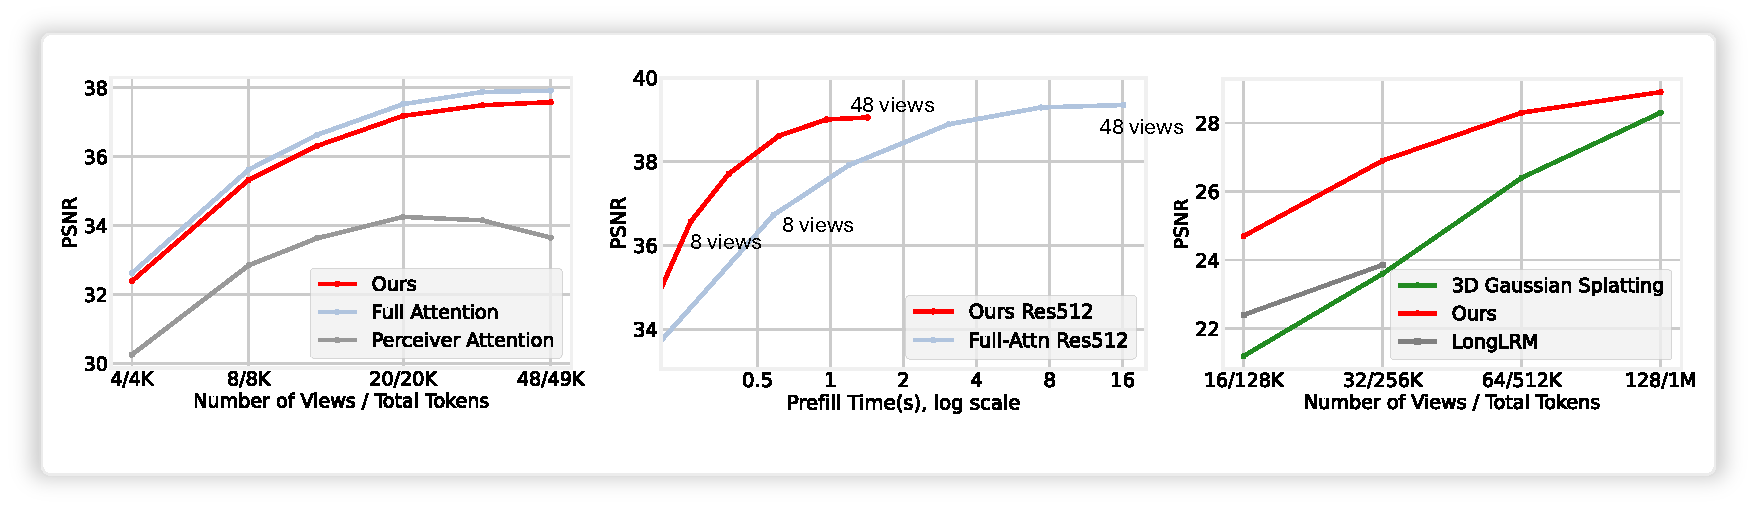
\includegraphics[width=\textwidth]{figures/figure_view_synthesis.pdf}
    \put(-345, 100){\capfontscriptsize GSO 256$\times$256}
    \put(-215, 100){\capfontscriptsize GSO 512$\times$512}
    \put(-100, 100){\capfontscriptsize DL3DV 960$\times$536}
    \put(-355,11){\capfont  \textbf{(a)} Object dataset }
    \put(-260,11){\capfont \textbf{(b)} Performance v.s. Prefill speed}
    \put(-130,11){\capfont \textbf{(c)} Scene dataset with 1M tokens}
    \vspace{-0.15in}
    \caption{\textbf{(a, b)} our method achieves quality comparable to full-attention models with significantly lower prefill latency,  and it clearly outperforms perceiver-attention baselines. \textbf{(c)} On the high resolution scene dataset, our approach surpasses LongLRM, limited to 32 views, and outperforms 3D Gaussian Splatting with sparse views, remaining competitive up to 128 input views (1M total tokens). }
    \vspace{-0.14in}
    \label{fig:view_syn_results}
\end{figure}

 
\subsection{Language Modeling}\label{sec:exp_language}

\noindent\textbf{Datasets \& Metrics.}
We train our models on the Long-Data-Collections dataset~\cite{long_data_collection}, using approximately 60B tokens from its total 68.8B tokens. For evaluation, we employ the per-token loss metric from~\cite{linforgetting}, assessing models' ability to effectively use the full context. A monotonically decreasing loss indicates successful context utilization, whereas plateauing suggests limited context usage. Additionally, we report retrieval accuracy~\cite{hsiehruler} at various sequence lengths.

%to assess each model's ability to memorize and retrieve relevant information from the context.


\noindent\textbf{Model details.} We remove the window-attention layer from the original the \methodname{} block, integrating a sliding window-attention(SWA) layer directly into the Large-Chunk TTT layer. Following GAU~\cite{hua2022transformer}, SWA shares Q, K, and V vectors with the fast-weight network, with additional per-channel scaling and shifting on Q and K. 
The pseudocode for this design is in Algorithm~\ref{alg:lact_hybrid}.
% See supplementary for pseudocode.

\noindent\textbf{Baselines.}
We compare against full attention, Gated Linear Attention (GLA)~\cite{yang2024gated}, DeltaNet~\cite{schlag2021linear,yangparallelizing}. To ensure fairness, we enhance both GLA and DeltaNet with the same sliding window attention. Based on prior work~\cite{linforgetting, xiong2023effective, men2024base} highlighting the importance of a large RoPE~\cite{su2023roformer} base for long-context transformer training,  we adopt a RoPE base of 1 million for training with 32K token contexts.
Tab.~\ref{tab:LM_baseline} summarize the mechanism and training throughput of all methods. 

\begin{table*}[t!]
\centering
\caption{Comparison of baseline methods in terms of state size, training throughput (measured in tokens per second, TPS), update rules, and memory read-out mechanisms. Training throughput is evaluated using a 3B-parameter model with 32K-sequence length on A100-40GB GPUs.}
\label{tab:LM_baseline}
\resizebox{\textwidth}{!}{%
\begin{tabular}{llllll}
\toprule
 & \textbf{State size}  & \textbf{Train TPS} &  \textbf{Update Rule} & \textbf{Memory read-out} \\
\midrule
Transformer     & –       & 4.1K     & – & – \\
Transformer SWA & –       & 6.4K   & – & – \\
\midrule
\multicolumn{5}{l}{ \textit{Per-token recurrence} } \\
GLA SWA         & $384d$  & 5.0K   &
$\displaystyle \mathbf{S}_t \leftarrow  \mathbf{S}_{t-1}\mathrm{Diag}(\boldsymbol{\alpha}_t) + \mathbf{v}_t \mathbf{k}_t^\top$ 
& $\displaystyle \mathbf{o}_t = \mathbf{S}_t \mathbf{q}_t$ \\
DeltaNet SWA    & $128d$  & 5.1K   &
$\displaystyle \mathbf{S}_t \leftarrow  \mathbf{S}_{t-1}(\mathbf{I} - \beta_t \mathbf{k}_t \mathbf{k}_t^\top) + \beta_t \mathbf{v}_t \mathbf{k}_t^\top$ 
& $\displaystyle \mathbf{o}_t = \mathbf{S}_t \mathbf{q}_t$ \\
\midrule
\multicolumn{5}{l}{ \textit{Large-chunk recurrence} } \\
Ours GD       & $2304d$ & 5.0K    
& $ W \leftarrow \mathrm{L2norm}(W - \sum_i^b \eta_i \nabla_W \mathcal{L}_i)$
& $\displaystyle \mathbf{o}_t = f_W(\mathbf{q}_t)$  \\
Ours  Momentum       & $2304d$ & 4.9K    
& $M \leftarrow \beta M + \sum_i^b \eta_i \nabla_W \mathcal{L}_i;\; W \leftarrow  \mathrm{L2norm}(W - M)$
& $\displaystyle \mathbf{o}_t = f_W(\mathbf{q}_t)$  \\
Ours Muon       & $2304d$ & 4.3K  
& $ M \leftarrow  \beta M + \sum_i^b \eta_i \nabla_W \mathcal{L}_i;\;  W \leftarrow  \mathrm{L2norm}(W - \mathrm{Muon}(M))$
& $\displaystyle \mathbf{o}_t = f_W(\mathbf{q}_t)$ \\
\bottomrule
\end{tabular}%
}
% \vspace{-0.4in}
\end{table*}

\noindent\textbf{Training details.} We trained models at two scales using a 32768-token sequence length: a 760M-parameter model trained for 40B tokens with a 2048-token sliding window, and a 3B-parameter model trained for 60B tokens with a 4096-token sliding window. See more details in Sec.~\ref{sec:appen_exp_language}.  
% Further details are in the Appendix.

\noindent\textbf{Results.} Please refer to Fig.~\ref{fig:lm_results} for experiment results and analysis. See more results in Sec.~\ref{sec:appen_exp_language}.
% \sai{
% We apply the per-token loss~\cite{linforgetting} to evaluate the long-context capability of each model.
% As pointed out in~\cite{linforgetting}, a monotonically decreasing per-token loss means the model 
% can make use of the full context well, while a plateaued loss at position $i$ means that the 
% model cannot make use of the information $i$ tokens away from the current position.  
% From Fig.~\ref{fig:lm_results}a, we can see that our model achieves comparable performance 
% to DeltaNet for token index $i<$6k, and slightly falls short of GLA, which is potentially because
% }

\begin{figure}[t!]
    \centering
    \vspace{-0.1in}
    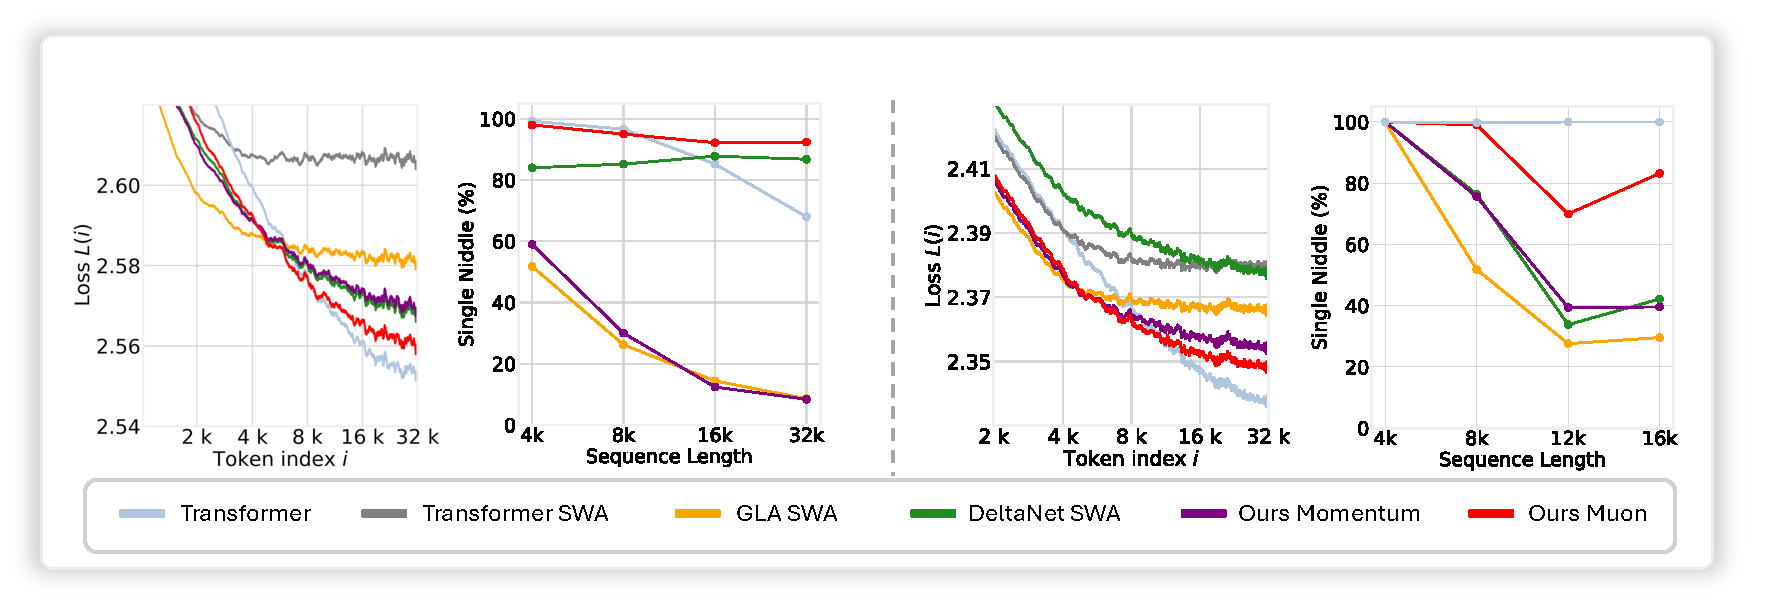
\includegraphics[width=\textwidth]{figures/figure_lm_result.pdf}
    \put(-388, 116){\capfont \textbf{(a)} 760M Validation loss}
    \put(-288, 116){\capfont \textbf{(b)} 760M S-NIAH-1}
    \put(-190, 116){\capfont \textbf{(c)} 3B Validaiton loss}
    \put(-94, 116){\capfont \textbf{(d)} 3B S-NIAH-2}
    \vspace{-0.1in}
    \caption{Language Model results. 
    \textbf{(a, c)} Our model achieves lower per-position loss at larger token indices compared to GLA and DeltaNet at both 760M and 3B scale, indicating stronger long-context modeling capability.
\textbf{(b, d)} Our model consistently outperforms GLA and DeltaNet in retrieval accuracy. Furthermore, our Muon variant consistently outperforms our Momentum variant.
    }
    \label{fig:lm_results}
    % \vspace{-0.1in}
\end{figure}



\subsection{Autoregressive Video Diffusion}\label{sec:exp_video}
We fine-tune the pretrained Wan 2.1~\cite{wang2025wan} text-to-video diffusion model into an autoregressive video diffusion model. Specifically, we replace all bidirectional attention layers with our \methodname{} layers combined with sliding window attention. The sliding window attention uses a window size spanning two autoregressive chunks.  

%We retain the original query-key-value (qkv) and output projections. 
% \yicong{For all models with window attention, the \methodname{} or Mamba2 layer is running in parallel with the sliding window attention, e.g., $x_{out} = \lambda_{LaCT} \cdot x_{LaCT} + x_{window}$, where $\lambda_{LaCT}$ is a learnable coefficient.}

\noindent\textbf{Datasets.} We fine-tune the model using an internal, filtered proprietary collection of videos, each accompanied by a short text prompt generated by a visual language model.

\noindent\textbf{Training details.}
Following~\cite{esser2403scaling, wang2025wan}, we employ time-step shifting and denoising loss weighting using a logit-normal distribution. we train on 5-second videos at 16 FPS and 480$\times$832 resolution, autoregressively denoising in 3 latent-frame chunks. Later we fine-tune the 1.3 billion parameter model with 10 second videos and 14 billion parameter model with 8.8 second videos. Each 8.8-second clip contains 56,160 visual tokens, resulting in interleaved noisy-clean chunks totaling 107K tokens under teacher-forcing training. We use sequence parallelism for MLP layers and tensor parallelism (sharding heads across devices) for TTT and window attention layers. Full details are listed in Sec.~\ref{sec:appen_exp_video}.


% We apply teacher-forcing training and formulate an interleaved noise-clean chunk sequence as input (see section~\ref{sec:method-arvideo}). This results in 39 latent frames comprising 7 noisy chunks and 6 clean chunks, totaling a sequence length of 60K tokens. Later we fine-tune the model with 8.8 second videos.  See supplementary for details.


\noindent\textbf{Baselines.}
We compare our method against three baselines: sliding window attention (SWA) alone, Mamba2~\cite{dao2024transformers} combined with SWA (using a similar parallel combination strategy as our method), and full block-wise causal attention.  
% Additional details are in the supplementary material.


\noindent\textbf{Evaluation.}
We evaluate all models on a collection of 2,000 videos after 5,000 training iterations by computing the denoising loss at five timesteps (550, 650, 750, 850, 950). 
Figure~\ref{fig:exp-video-baseline} plots the chunk-wise denoising loss across evaluated video frames. We only measure validation loss  up to training sequence length. See project website for our autoregressively generated videos \footnote{See video results in project website: \url{https://tianyuanzhang.com/projects/ttt-done-right/}}. 

\begin{figure}[t!]
    \centering
    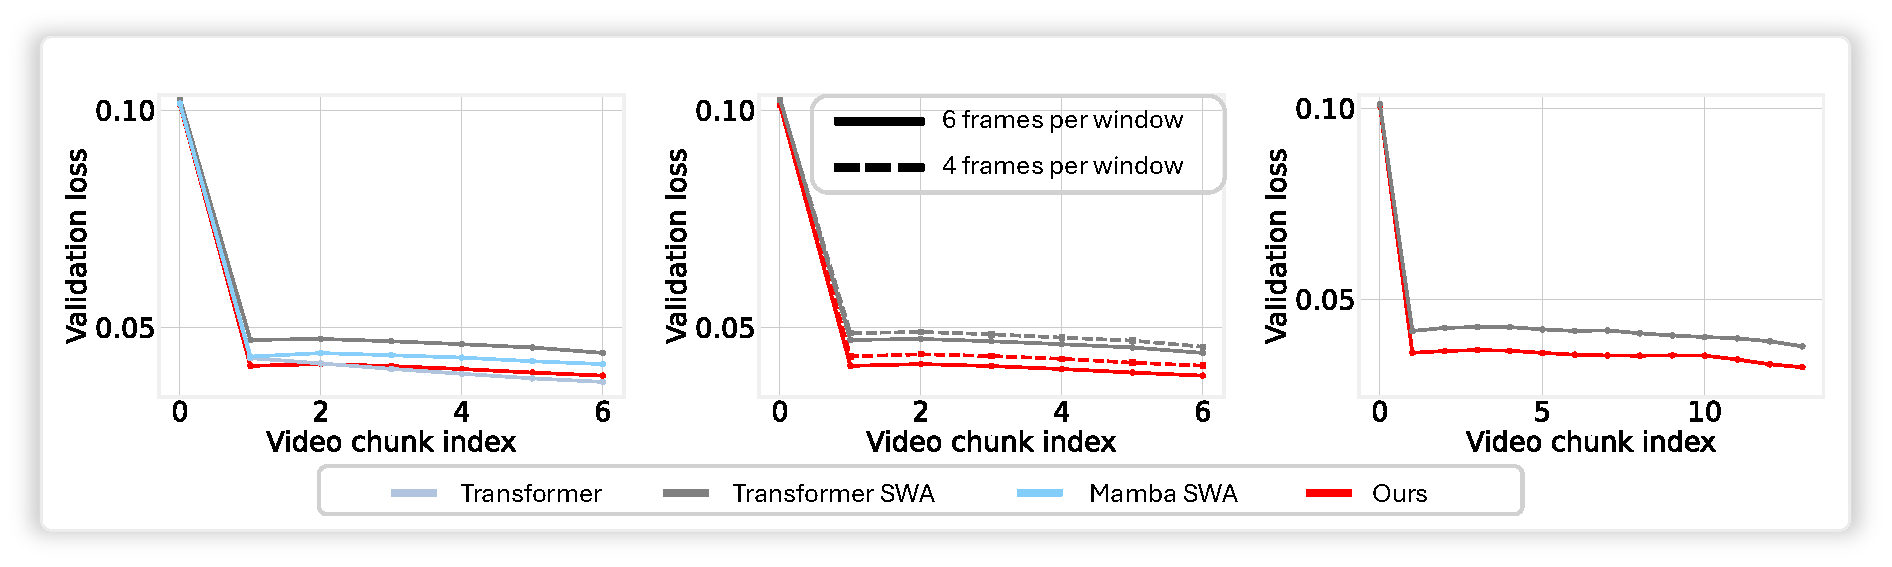
\includegraphics[width=\textwidth]{figures/figure_video_exp.pdf}
    \put(-376, 103){\capfont \textbf{(a)} Comparison with baselines}
    \put(-245, 103){\capfont \textbf{(b)} Ablate on window size}
    \put(-110, 103){\capfont \textbf{(c)} Eval on longer videos}
    \vspace{-1em}
    \caption{(a) We achieve comparable validation loss to the full-attention baseline and outperform both Mamba with sliding window and sliding window attention baselines. This improvement over SWA is consistent across different window sizes (b) and when evaluating on longer videos (c).}
    \label{fig:exp-video-baseline}
    \vspace{-0.2in}
\end{figure}



\subsection{Analysis on Design Choices}\label{sec:analysis}

% \subsubsection{Effects of Scaling State Size}
% \label{sec:exp-state-size-scaling}
% The size of the fast weight, or state size, affects the capacity of memory a lot. 
% We study its effects by scaling it up on the novel view synthesis task and language model task at a 760 million parameter scale. Making figure here. 
% In this section, we analyze several key design choices in our model, focusing on both the novel view synthesis and language modeling tasks. Specifically, we evaluate the 
% impact of state size (Fig.~\ref{fig:exp-state-optimizer}a), 
% test-time optimizers (Fig.~\ref{fig:exp-state-optimizer}b),
% linear versus nonlinear fast weights(Fig.~\ref{fig:exp-linear-token-recurrence}a), and 
% per-token recurrence versus chunk-wise recurrence (Fig.~\ref{fig:exp-linear-token-recurrence}b). Please refer to Appendix~\ref{appendix_sec:analysis} for results and conclusions. 



In this section, we analyze several key design choices in our model, focusing on both the novel view synthesis and language modeling tasks, where good metrics exist. Specifically, we evaluate the 
impact of state size (Fig.~\ref{fig:exp-state-optimizer}a), 
test-time optimizers (Fig.~\ref{fig:exp-state-optimizer}b),
linear versus nonlinear fast weights (Fig.~\ref{fig:exp-linear-token-recurrence}a), and 
per-token recurrence versus chunk-wise recurrence (Fig.~\ref{fig:exp-linear-token-recurrence}b).
Overall, we find that a large state size, advanced optimizers such as Muon, and nonlinear fast weights significantly improve our model’s performance. For comparing chunk recurrence with per-token recurrence, in a controlled NVS experiment, our linear large-chunk recurrence strategy outperforms linear per-token recurrence with the same state size. For language modeling, where chunk structures are not inherent, our linear large-chunk recurrence variant—while initially underperforming per-token methods like GLA and DeltaNet—surpasses them when combined with a large nonlinear state and the Muon optimizer.
We refer the readers to each figure and its caption for more detailed analysis. 


\begin{figure}[htbp]
    \centering
    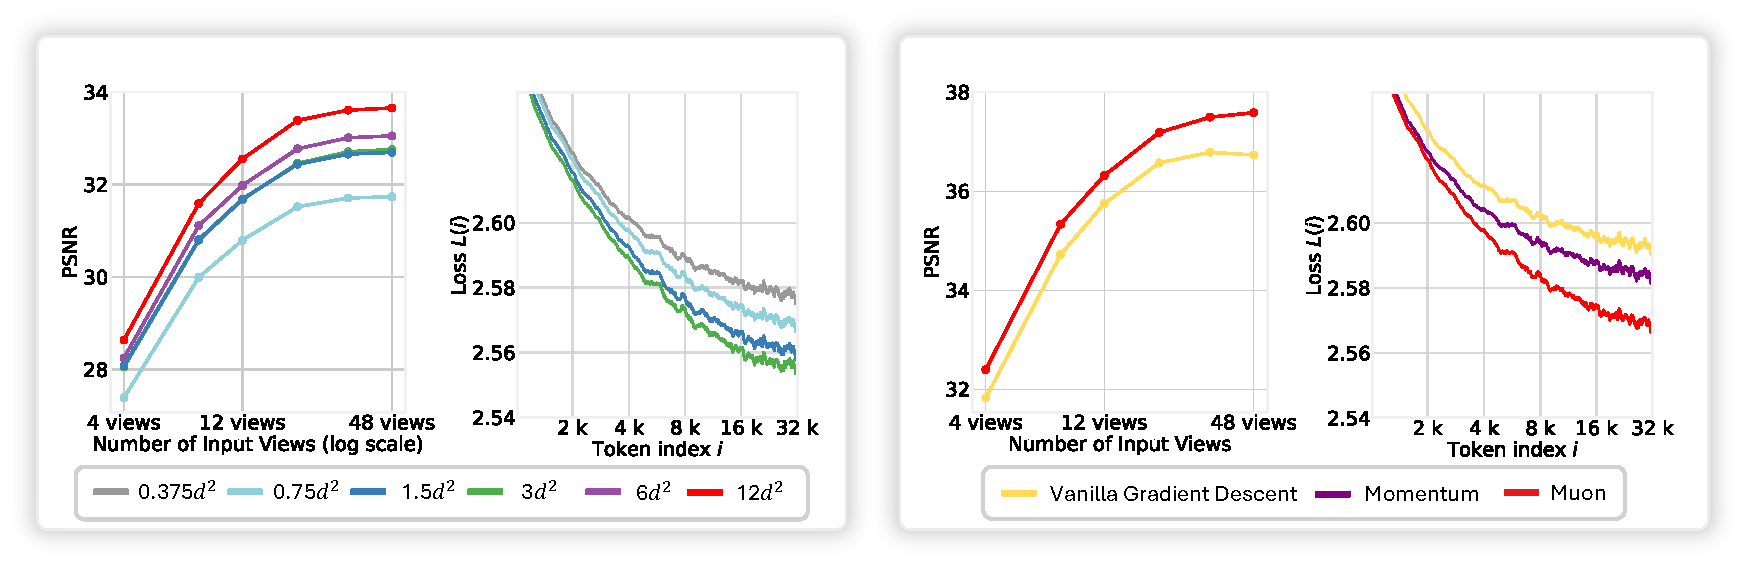
\includegraphics[width=\textwidth]{figures/figure_exp_state_optimizer.pdf}
    \put(-373, 113){\capfontscriptsize novel view synthesis}
    \put(-268, 113){\capfontscriptsize language model}
    \put(-173, 113){\capfontscriptsize novel view synthesis}
    \put(-70, 113){\capfontscriptsize language model}
    \put(-330, -5){\capfont \textbf{(a)} State Size Scaling}
    \put(-160, -5){\capfont \textbf{(b)} Different Test-Time optimizer}
    \caption{ \textbf{(a)} Scaling up the state size consistently improves performance in both novel view synthesis and language modeling tasks. Note, the largest version has state size of $12d^2$ per block, totaling 40\% of model weights as fast weights. \textbf{(b)} Comparison of test-time optimizers demonstrates Muon’s surprising effectiveness over Vanilla Gradient Descent and Momentum. }
    \label{fig:exp-state-optimizer}
\end{figure}







\begin{figure}[htbp]
    \centering
    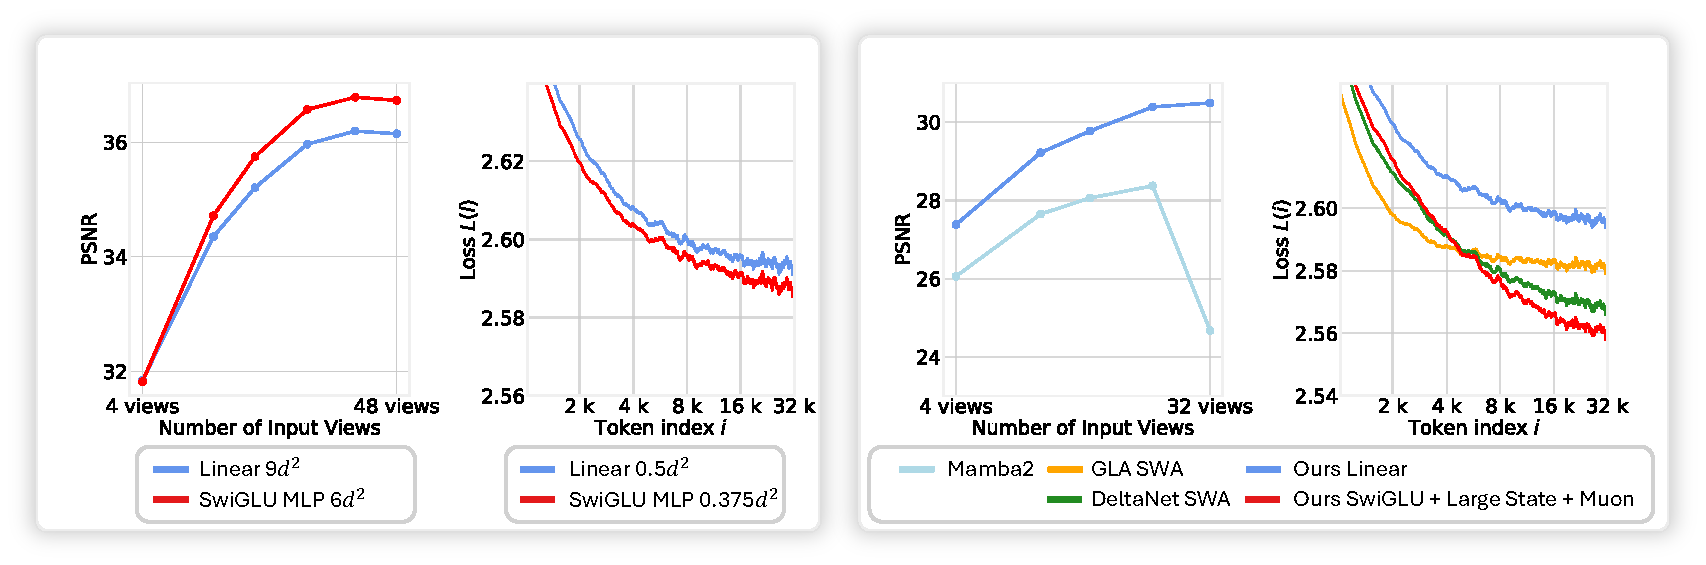
\includegraphics[width=0.99\textwidth]{figures/figure_exp_linear_token_recurrence.pdf}
    \put(-360, 115){\capfontscriptsize novel view synthesis}
    \put(-262, 115){\capfontscriptsize language model}
    \put(-173, 115){\capfontscriptsize novel view synthesis}
    \put(-75, 115){\capfontscriptsize language model}
    \put(-360,-5){\capfont \textbf{(a)} Linear v.s. NonLinear Fast weight}
    \put(-176,-5){\capfont \textbf{(b)} Large-Chunk v.s. Per-token Recurrence}
    \caption{\textbf{(a)} Nonlinear fast weights consistently outperform linear fast weights despite using smaller state sizes. \textbf{(b)} Our linear large-chunk recurrence approach significantly outperforms linear per-token recurrence (bidirectional Mamba2) for view synthesis tasks at the same state sizes.  In language tasks, linear large-chunk recurrence of the same state size underperforms the GLA baseline, but when combined with larger nonlinear states and Muon test-time optimizer, it surpasses all per-token recurrence methods.}
    \label{fig:exp-linear-token-recurrence}
\end{figure}


\paragraph{State size scaling.} 
% The analyses in this section used the following experiment configurations:
These controlled experiments utilize a SwiGLU MLP for fast weights and the Muon as the test-time optimizer.
For NVS, experiments were conducted on the object dataset. All models were trained for 167B tokens, using 14 stacked blocks and a model dimension $d=768$. To change the state size, we keep the head dimension fixed as model dimension. i.e. single head, and vary the intermediate dimension of SwiGLU MLP, such that the intermediate dimension ranges from $192$ to $3072$. The largest configuration results in a state size per model block as $12d^2$, totaling $40\%$ of model weights as fast weights.  For the language model experiments, we use the 760 milion parameter setup, where the chunk size and sliding window attention (SWA) window size were set to 2048 tokens. We keep the intermediate dimension of the fast weight SwiGLU MLP the same as the head dimension. We increase the state size while proportionally decreasing the number of heads to maintain a fixed model dimension. Figure~\ref{fig:exp-state-optimizer}(a) demonstrates that larger state sizes consistently improve performance. Notably, the performance gap between small and large state sizes widens with increasing sequence length.


\paragraph{Test-Time optimizer comparison. }
We compare Muon with vanilla Gradient Descent (GD) and GD with momentum. Details on momentum implementation are in Appendix~\ref{paragraph:momentum}.   For NVS, we train all compared approaches for 671 tokens using model specs of 24 stacked blocks with model dimension of 768. Language modeling experiments used the 760M parameter setup. Figure~\ref{fig:exp-state-optimizer}(b) shows Muon consistently outperforming other optimizers.


\paragraph{Linear v.s. NonLinear fast weight.} Our default fast weight function is a SwiGLU MLP without bias terms (nonlinear). We compare this against a simple linear fast weight, $f_W(x) = Wx$. Both are updated using the same online dot product loss for key-value association. Figure~\ref{fig:exp-linear-token-recurrence} (a) presents this comparison for NVS and language modeling. Although the linear fast weights were configured with a larger state size than the nonlinear SwiGLU, they achieved lower performance.  NVS models were trained for 671B tokens with 24 blocks and $d=768$.  Language modeling used the 760M parameter setup.



\paragraph{Large-chunk v.s. Per-token recurrence.} 
Figure~\ref{fig:exp-linear-token-recurrence}(b) presents controlled experiments comparing our large-chunk recurrence with per-token recurrence. 
In the novel view synthesis (NVS) task, ``Our Linear" variant employs a linear fast weight: $f_W(x) = Wx$ and is benchmarked against a Mamba-2 baseline (a linear per-token recurrence model) with an identical state size. To accommodate the bidirectional context required by NVS over input image tokens, the Mamba-2 baseline uses two Mamba-2 layers applied in opposite directions within each model block. Both our linear variant and this bidirectional Mamba-2 have state size of $d^2$ per block. Both of these two approaches employs a per-image window attention within each model block. Under this fair comparison, our linear large-chunk recurrence achieves significantly better view synthesis performance.

For the language modeling experiments also shown in Figure~\ref{fig:exp-linear-token-recurrence}(b), the blue line ``Our Linear" variant uses the same state size ($0.25 d^2$) as the GLA SWA baseline. It initially underperforms GLA SWA (blue line underperforms yellow line),  likely because language data lacks the inherent chunk structures that benefit our basic linear chunk recurrence. However, when LaCT is equipped with a larger non-linear state ($1.5d^2$) and Muon updates, we significantly outperform these per-token recurrence baselines.

